%
% This is the LaTeX template file for lecture notes for EE 382C/EE 361C.
%
% To familiarize yourself with this template, the body contains
% some examples of its use.  Look them over.  Then you can
% run LaTeX on this file.  After you have LaTeXed this file then
% you can look over the result either by printing it out with
% dvips or using xdvi.
%
% This template is based on the template for Prof. Sinclair's CS 270.

\documentclass[twoside]{article}
\usepackage{graphics}
\setlength{\oddsidemargin}{0.25 in}
\setlength{\evensidemargin}{-0.25 in}
\setlength{\topmargin}{-0.6 in}
\setlength{\textwidth}{6.5 in}
\setlength{\textheight}{8.5 in}
\setlength{\headsep}{0.75 in}
\setlength{\parindent}{0 in}
\setlength{\parskip}{0.1 in}

%
% The following commands set up the lecnum (lecture number)
% counter and make various numbering schemes work relative
% to the lecture number.
%
\newcounter{lecnum}
\renewcommand{\thepage}{\thelecnum-\arabic{page}}
\renewcommand{\thesection}{\thelecnum.\arabic{section}}
\renewcommand{\theequation}{\thelecnum.\arabic{equation}}
\renewcommand{\thefigure}{\thelecnum.\arabic{figure}}
\renewcommand{\thetable}{\thelecnum.\arabic{table}}

%
% The following macro is used to generate the header.
%
\newcommand{\lecture}[4]{
	\pagestyle{myheadings}
	\thispagestyle{plain}
	\newpage
	\setcounter{lecnum}{#1}
	\setcounter{page}{1}
	\noindent
	\begin{center}
		\framebox{
			\vbox{\vspace{2mm}
				\hbox to 6.28in { {\bf EE 382C/361C: Multicore Computing
						\hfill Fall 2016} }
				\vspace{4mm}
				\hbox to 6.28in { {\Large \hfill Lecture #1: #2  \hfill} }
				\vspace{2mm}
				\hbox to 6.28in { {\it Lecturer: #3 \hfill Scribe: #4} }
				\vspace{2mm}}
		}
	\end{center}
	\markboth{Lecture #1: #2}{Lecture #1: #2}
	%{\bf Disclaimer}: {\it These notes have not been subjected to the
	%usual scrutiny reserved for formal publications.  They may be distributed
	%outside this class only with the permission of the Instructor.}
	\vspace*{4mm}
}

%
% Convention for citations is authors' initials followed by the year.
% For example, to cite a paper by Leighton and Maggs you would type
% \cite{LM89}, and to cite a paper by Strassen you would type \cite{S69}.
% (To avoid bibliography problems, for now we redefine the \cite command.)
% Also commands that create a suitable format for the reference list.
\renewcommand{\cite}[1]{[#1]}
\def\beginrefs{\begin{list}%
		{[\arabic{equation}]}{\usecounter{equation}
			\setlength{\leftmargin}{2.0truecm}\setlength{\labelsep}{0.4truecm}%
			\setlength{\labelwidth}{1.6truecm}}}
	\def\endrefs{\end{list}}
\def\bibentry#1{\item[\hbox{[#1]}]}

%Use this command for a figure; it puts a figure in wherever you want it.
%usage: \fig{NUMBER}{SPACE-IN-INCHES}{CAPTION}
\newcommand{\fig}[3]{
	\vspace{#2}
	\begin{center}
		Figure \thelecnum.#1:~#3
	\end{center}
}
% Use these for theorems, lemmas, proofs, etc.
\newtheorem{theorem}{Theorem}[lecnum]
\newtheorem{lemma}[theorem]{Lemma}
\newtheorem{proposition}[theorem]{Proposition}
\newtheorem{claim}[theorem]{Claim}
\newtheorem{corollary}[theorem]{Corollary}
\newtheorem{definition}[theorem]{Definition}
\newenvironment{proof}{{\bf Proof:}}{\hfill\rule{2mm}{2mm}}

% **** IF YOU WANT TO DEFINE ADDITIONAL MACROS FOR YOURSELF, PUT THEM HERE:
\usepackage{listings}
\usepackage{graphicx}
\begin{document}
	%FILL IN THE RIGHT INFO.
	%\lecture{**LECTURE-NUMBER**}{**DATE**}{**LECTURER**}{**SCRIBE**}
	\lecture{19}{November 1}{Vijay Garg}{Yue Zhao}
	%\footnotetext{These notes are partially based on those of Nigel Mansell.}
	
	% **** YOUR NOTES GO HERE:
	
	% Some general latex examples and examples making use of the
	% macros follow.  
	%**** IN GENERAL, BE BRIEF. LONG SCRIBE NOTES, NO MATTER HOW WELL WRITTEN,
	%**** ARE NEVER READ BY ANYBODY.
	\section{Wait Free Consensus Hierachy}
	
	Consensus number of a shared object is the maximum number of processes that can use that object to solve consensus problem.
	
	Operation:
	R/W Register: Consensus number 1;\\
	TestAndSet: Consensus number 2;\\
	GetAndIncrement: Consensus number 2;\\
	Swap: Consensus number 2;\\
	CAS: Consensus number infinity;\\
	\subsection{Read-Modify-Write Objects}
	An Read-Modify-Write Object has the following structure:
	\begin{center}
		\begin{lstlisting}[language=Java]
		private int value; 
		public int synchronized getAndModify(int x) {
		int prev = value;
		value = f(value, x);
		return prev;
		}
		\end{lstlisting}
	\end{center}
	
	Function f sets a new value and returns the old value:
	\begin{itemize}
		\item Test\&Set: f(value, x) = 1;
		\item Swap:  f(value, x) = x;
		\item Get\&Increment: f(value, x) = value+1;
	\end{itemize}
	
	An read-and-modify object can be characterized by function f:\\
	(1) RMW is commute if: fi fj = fj fi (for any i, j), where fi is the function applied by process i;\\
	(2) RMW is overwrite if: fi(fj(x)) = fi(x) (for any i, j);
	
	Theorem:\\
	Any \textbf{non-trivial} (f is not identity, if f is idenity, f is read operation f(value, x) = value, which has consensus number 1) RMW object with either commuting or overwriting property has consensus number equals to two.
	
	Proof(consensus number is at least 2):\\
	Use non-triviality: Value init to null. P0 and P1 store their proposals to an int[2] array.  There exists value such that f(value)!=value. Then call RMW, if return initial value then choose my value; else choose the other value;
	
	Proof(consensus number is at most 2):\\
	There is no protocol that solves consensus for 3 processes using RMW object. Any protocol has to reach some critical state:
	
	\begin{center}
		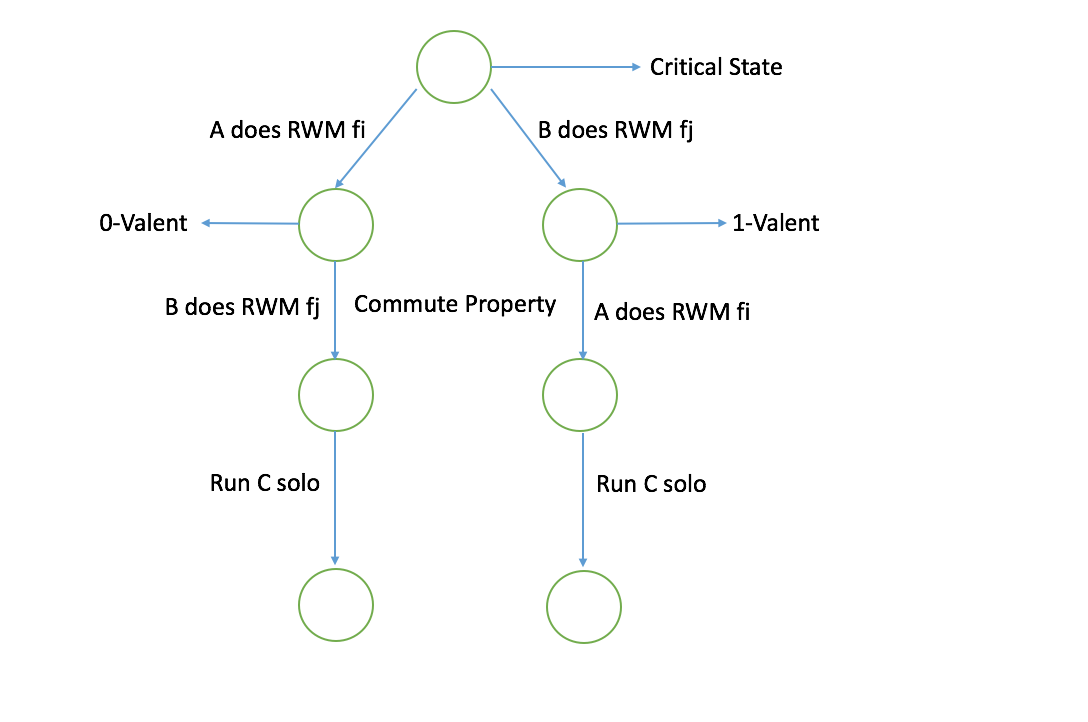
\includegraphics[scale=0.7]{upload.png}
	\end{center}
	
	From critical state, A does RMW(fi) reach 0-valent then B does RMW(fj); for another path, B does RMW(fj) reach 1-valent then A does RMW(fj). Because RMW has commute property, these two path has same state, then C can run. For C, the initial state is same, so, C will always reach same consensus and it cannot decide on different things. However, for the first path, C should reach 0-valent and for the second path, C should reach 1-valent, which contradict with uni-valent property.
	
	
	\subsection{2-Write-1-Read-Object ((2, 1) Object)}
	2-Write-1-Read-Object: Write on two locations atomically, read any one location.\\
	Protocol to solve consensus using (2, 1) object:\\
	
	int[3] (initial with null);\\
	Write proposal on int[3] array;\\
	P0 writes (a, a) in location 0 and 1;\\
	P1 writes (b, b) in location 1 and 2;\\
	Whichever writes first wins.
	
	Possible configurations during the process:\\
	\{a, a, null\}, (P0 won at this point);\\
	\{a, b, b\}, (P0 won);\\
	\{null, b, b\}, (P1 won);\\
	\{a, a, b\} (P1 won);\\
	
	This can solve consensus on 2 processes.
	
	\section{Universal Construction}
	Given some objects of consensus number m, construct an object with consensus number less than or equal to M.\\
	\textbf{Deterministic Objects:} state + operation cause a deterministic state.\\
	Universal Construction only applies to deterministic state.\\
	Correct Way: use a LinkedList, see code in github
	Initail state(Tail) -\textgreater apply method1 -\textgreater apply method2 -\textgreater apply method3(head) \\
	Each time invoking a method, add a node in the linkedlist as the new head.
	
	\section{Hashing}
	
	\begin{center}
		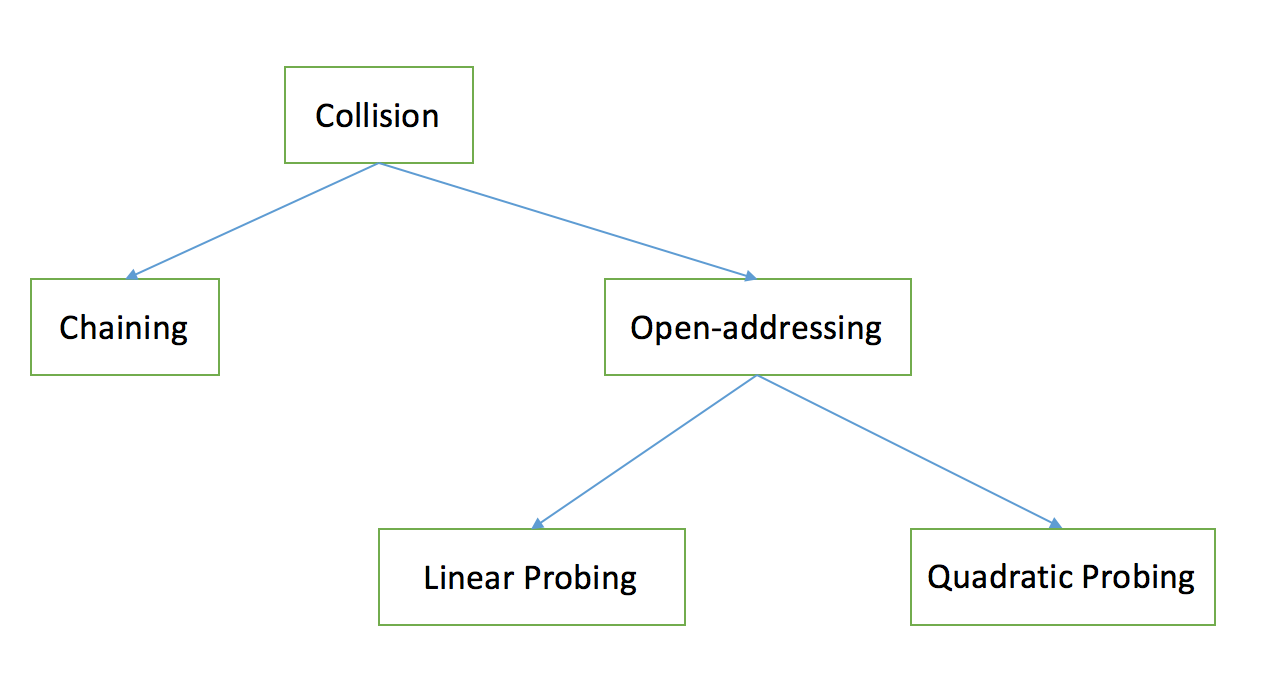
\includegraphics[scale=0.7]{hashing.png}
	\end{center}
	
	Linear Probing: insert in the next empty slot. May cause clustering effect and damage performance. \\
	Quadratic Probing: Try h(i) -\textgreater h(i)+1 -\textgreater h(i)+2^2 -\textgreater h(i)+3^2 -\textgreater h(i)+4^2 \\
	
	\textbf{Parallel Chaining:}
	\begin{center}
		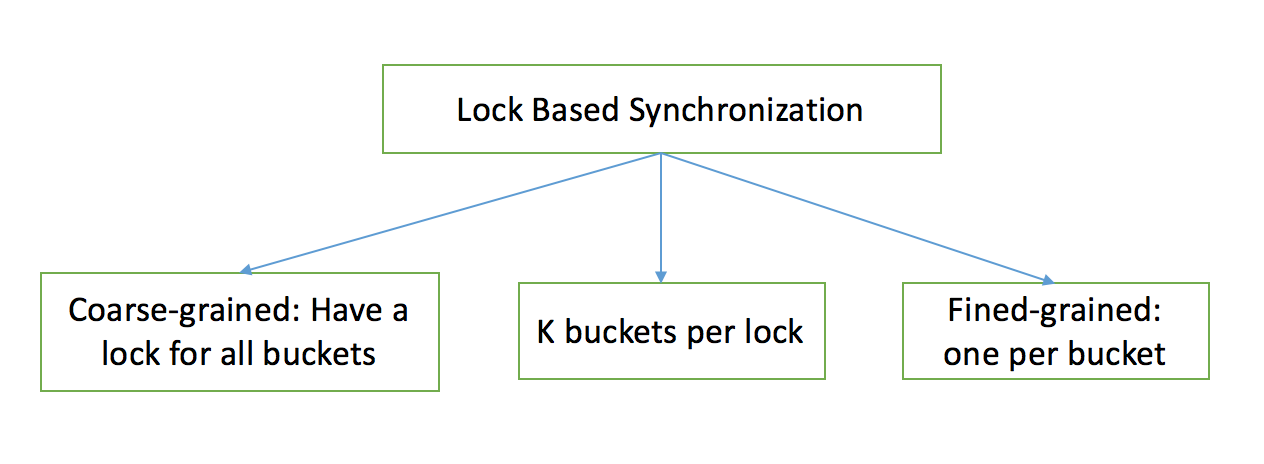
\includegraphics[scale=0.7]{parallelHashing.png}
	\end{center}
	
\end{document}





